% Options for packages loaded elsewhere
\PassOptionsToPackage{unicode}{hyperref}
\PassOptionsToPackage{hyphens}{url}
%
\documentclass[
  10pt,
  ignorenonframetext,
]{beamer}
\usepackage{pgfpages}
\setbeamertemplate{caption}[numbered]
\setbeamertemplate{caption label separator}{: }
\setbeamercolor{caption name}{fg=normal text.fg}
\beamertemplatenavigationsymbolsempty
% Prevent slide breaks in the middle of a paragraph
\widowpenalties 1 10000
\raggedbottom
\setbeamertemplate{part page}{
  \centering
  \begin{beamercolorbox}[sep=16pt,center]{part title}
    \usebeamerfont{part title}\insertpart\par
  \end{beamercolorbox}
}
\setbeamertemplate{section page}{
  \centering
  \begin{beamercolorbox}[sep=12pt,center]{part title}
    \usebeamerfont{section title}\insertsection\par
  \end{beamercolorbox}
}
\setbeamertemplate{subsection page}{
  \centering
  \begin{beamercolorbox}[sep=8pt,center]{part title}
    \usebeamerfont{subsection title}\insertsubsection\par
  \end{beamercolorbox}
}
\AtBeginPart{
  \frame{\partpage}
}
\AtBeginSection{
  \ifbibliography
  \else
    \frame{\sectionpage}
  \fi
}
\AtBeginSubsection{
  \frame{\subsectionpage}
}
\usepackage{amsmath,amssymb}
\usepackage{lmodern}
\usepackage{iftex}
\ifPDFTeX
  \usepackage[T1]{fontenc}
  \usepackage[utf8]{inputenc}
  \usepackage{textcomp} % provide euro and other symbols
\else % if luatex or xetex
  \usepackage{unicode-math}
  \defaultfontfeatures{Scale=MatchLowercase}
  \defaultfontfeatures[\rmfamily]{Ligatures=TeX,Scale=1}
\fi
% Use upquote if available, for straight quotes in verbatim environments
\IfFileExists{upquote.sty}{\usepackage{upquote}}{}
\IfFileExists{microtype.sty}{% use microtype if available
  \usepackage[]{microtype}
  \UseMicrotypeSet[protrusion]{basicmath} % disable protrusion for tt fonts
}{}
\makeatletter
\@ifundefined{KOMAClassName}{% if non-KOMA class
  \IfFileExists{parskip.sty}{%
    \usepackage{parskip}
  }{% else
    \setlength{\parindent}{0pt}
    \setlength{\parskip}{6pt plus 2pt minus 1pt}}
}{% if KOMA class
  \KOMAoptions{parskip=half}}
\makeatother
\usepackage{xcolor}
\newif\ifbibliography
\setlength{\emergencystretch}{3em} % prevent overfull lines
\providecommand{\tightlist}{%
  \setlength{\itemsep}{0pt}\setlength{\parskip}{0pt}}
\setcounter{secnumdepth}{-\maxdimen} % remove section numbering
\usepackage{booktabs}

\usepackage{color, colortbl}
\definecolor{Gray}{gray}{0.9}

\def\begincols{\begin{columns}}
\def\begincol{\begin{column}}
\def\endcol{\end{column}}
\def\endcols{\end{columns}}

\setbeamertemplate{caption}[numbered]
\setbeamertemplate{itemize items}[default]
\setbeamertemplate{itemize subitem}[circle]

\logo{
\includegraphics[scale=0.2]{bbk200}}
%\usetheme{Madrid}
%\usefonttheme{serif}

%\pgfdeclareimage[scale=0.2]{logo}{bbk2}
%\logo{\pgfuseimage{logo}}

% \begincols
% \begincol{.48\textwidth}
% \endcol
% \begincol{.48\textwidth}
% \endcol
% \endcols

% How many criminal candidates were there? Where and when?
% 6,499 out of 35,075 contesting candidates -- close to 20\%

% Did criminal candidates win elections? Where and when?
% Given that a candidate is a criminal, the probability of winning the election is about 0.22; in contrast, Given that a candidate is NOT a criminal, the probability of winning the election is about 0.12. (X)

% How many criminal politicians were there? Where and when? 

% Party affiliations: BJP (23\%), Congress (18\%), 
\ifLuaTeX
  \usepackage{selnolig}  % disable illegal ligatures
\fi
\IfFileExists{bookmark.sty}{\usepackage{bookmark}}{\usepackage{hyperref}}
\IfFileExists{xurl.sty}{\usepackage{xurl}}{} % add URL line breaks if available
\urlstyle{same} % disable monospaced font for URLs
\hypersetup{
  hidelinks,
  pdfcreator={LaTeX via pandoc}}

\title{\hfill\break
\hfill\break
CP\(^2\) Week 2: From Empire to Nation-State\\
\strut \\}
\author{Dr Chao-Yo Cheng\\}
\date{}

\begin{document}
\frame{\titlepage}

\begin{frame}{Recap: Studying Chinese politics in the changing world}
\protect\hypertarget{recap-studying-chinese-politics-in-the-changing-world}{}
\begin{itemize}
  \item From intelligence services to academic research
  \vspace{0.5cm}
  \item From area studies to comparative politics
  \vspace{0.5cm}
  \item From qualitative description to data-intensive inference
\end{itemize}
\end{frame}

\begin{frame}
\begin{itemize}
  \item From intelligence services to new geopolitcal tension
  \vspace{0.1cm}
  \begin{itemize}
    \item China studies $\neq$ Sinology; emerging as a subject area after the WWII and gain its prominence during the Cold War
    \item "Echo chambers" in the making -- the changing geopolitical landscape in the past decade may drag China scholars in different countries to focus on different agenda
  \end{itemize}
  \vspace{0.3cm}
  \item From area studies to comparative politics
  \vspace{0.3cm}
  \item From qualitative description to data-intensive inference
\end{itemize}
\end{frame}

\begin{frame}
\begin{center}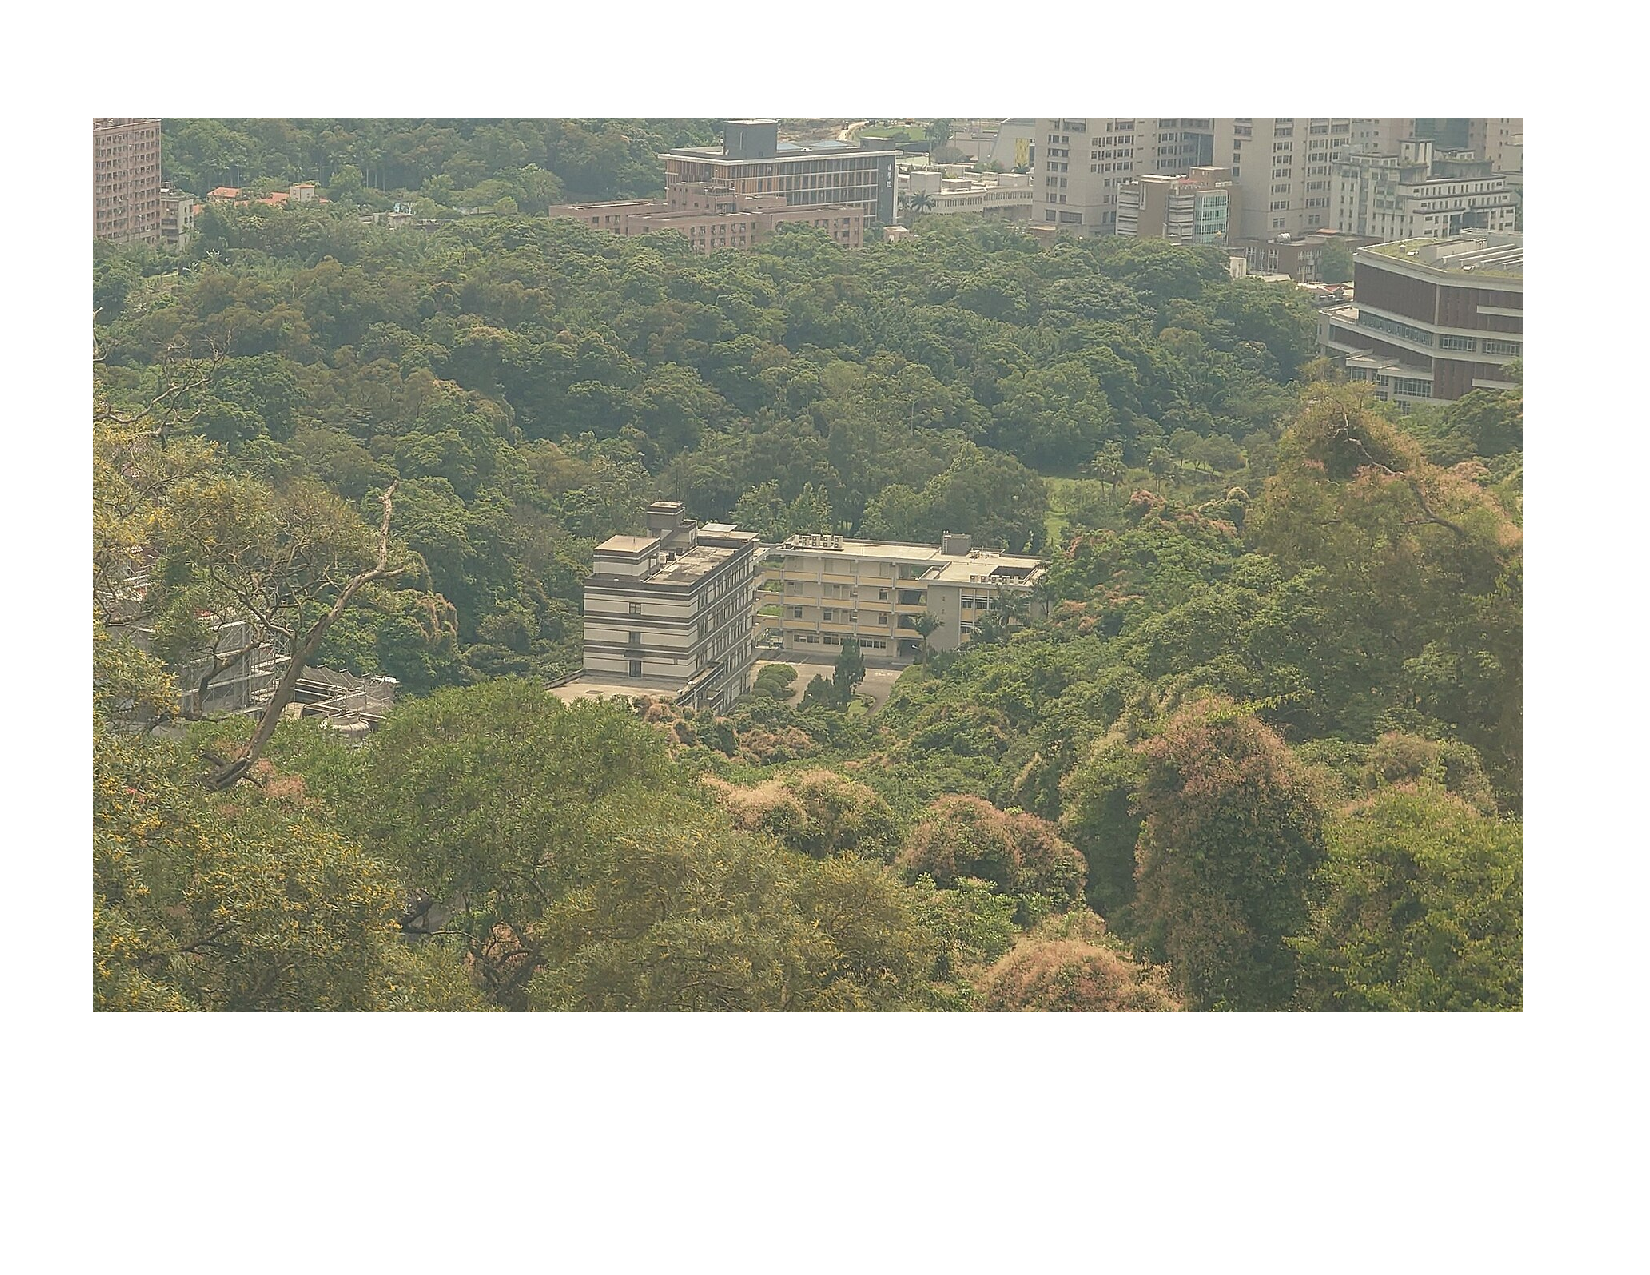
\includegraphics[width=0.8\linewidth]{Figs/nccu} \end{center}
\vspace{0.3cm}
\begin{center}
\small
Institute of International Relations, National Chengchi University (Taipei)
\end{center}
\end{frame}

\begin{frame}
\begin{itemize}
  \item From intelligence services to academic research
  \vspace{0.3cm}
  \item From area studies to comparative politics
  \vspace{0.1cm}
  \begin{itemize}
    \item Earlier generations of China scholars treat China as a distinct subfield within political science
    \item Later on, China scholars begin to borrow or "stretch" concepts and ideas from other subfields to study Chinese politics (Shambaugh 2023)
    \item Starting from the late 2000s, China scholars are about to generate new theoretical insights to general political science (Tsai 2017)
  \end{itemize}
  \vspace{0.3cm}
  \item From qualitative description to data-intensive inference
\end{itemize}
\end{frame}

\begin{frame}
\begin{center}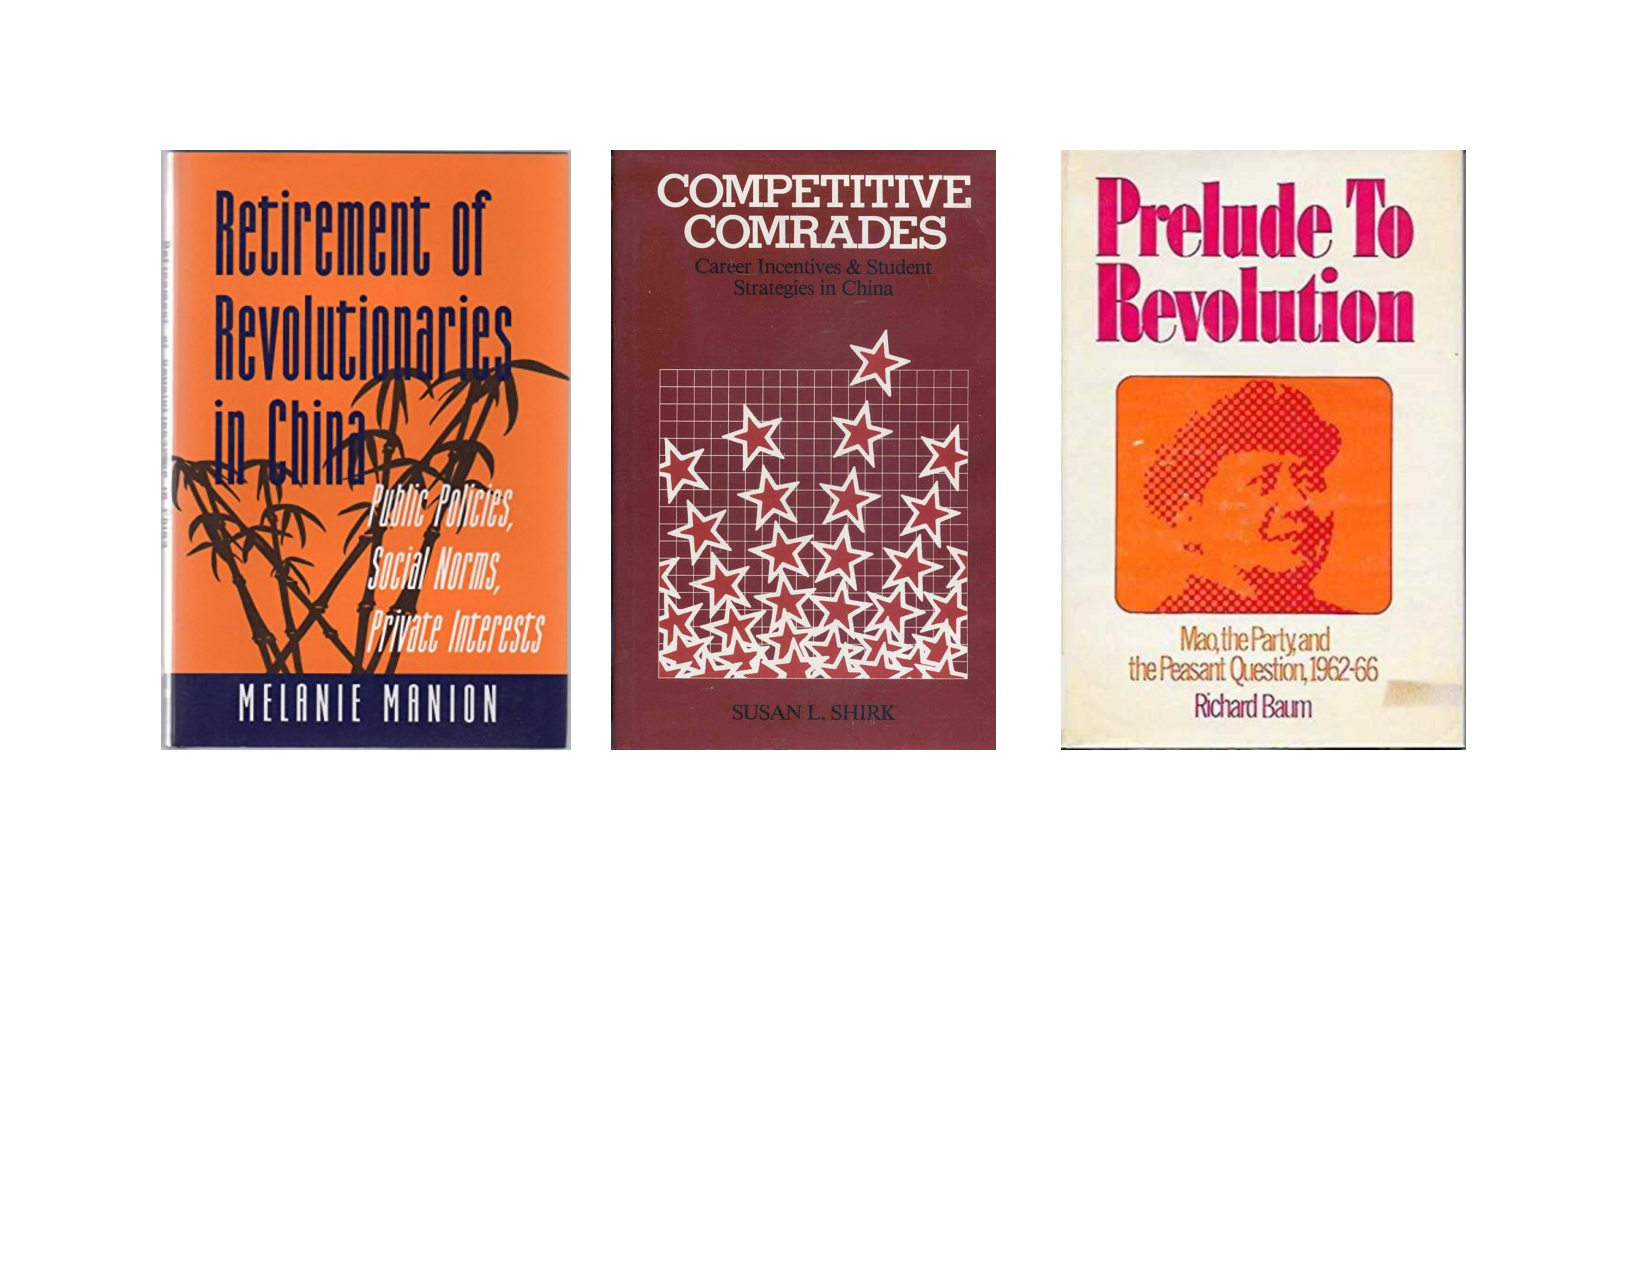
\includegraphics[width=1\linewidth]{Figs/book1} \end{center}
\end{frame}

\begin{frame}
\begin{center}\includegraphics[width=1\linewidth]{Figs/book2} \end{center}
\end{frame}

\begin{frame}
\begin{center}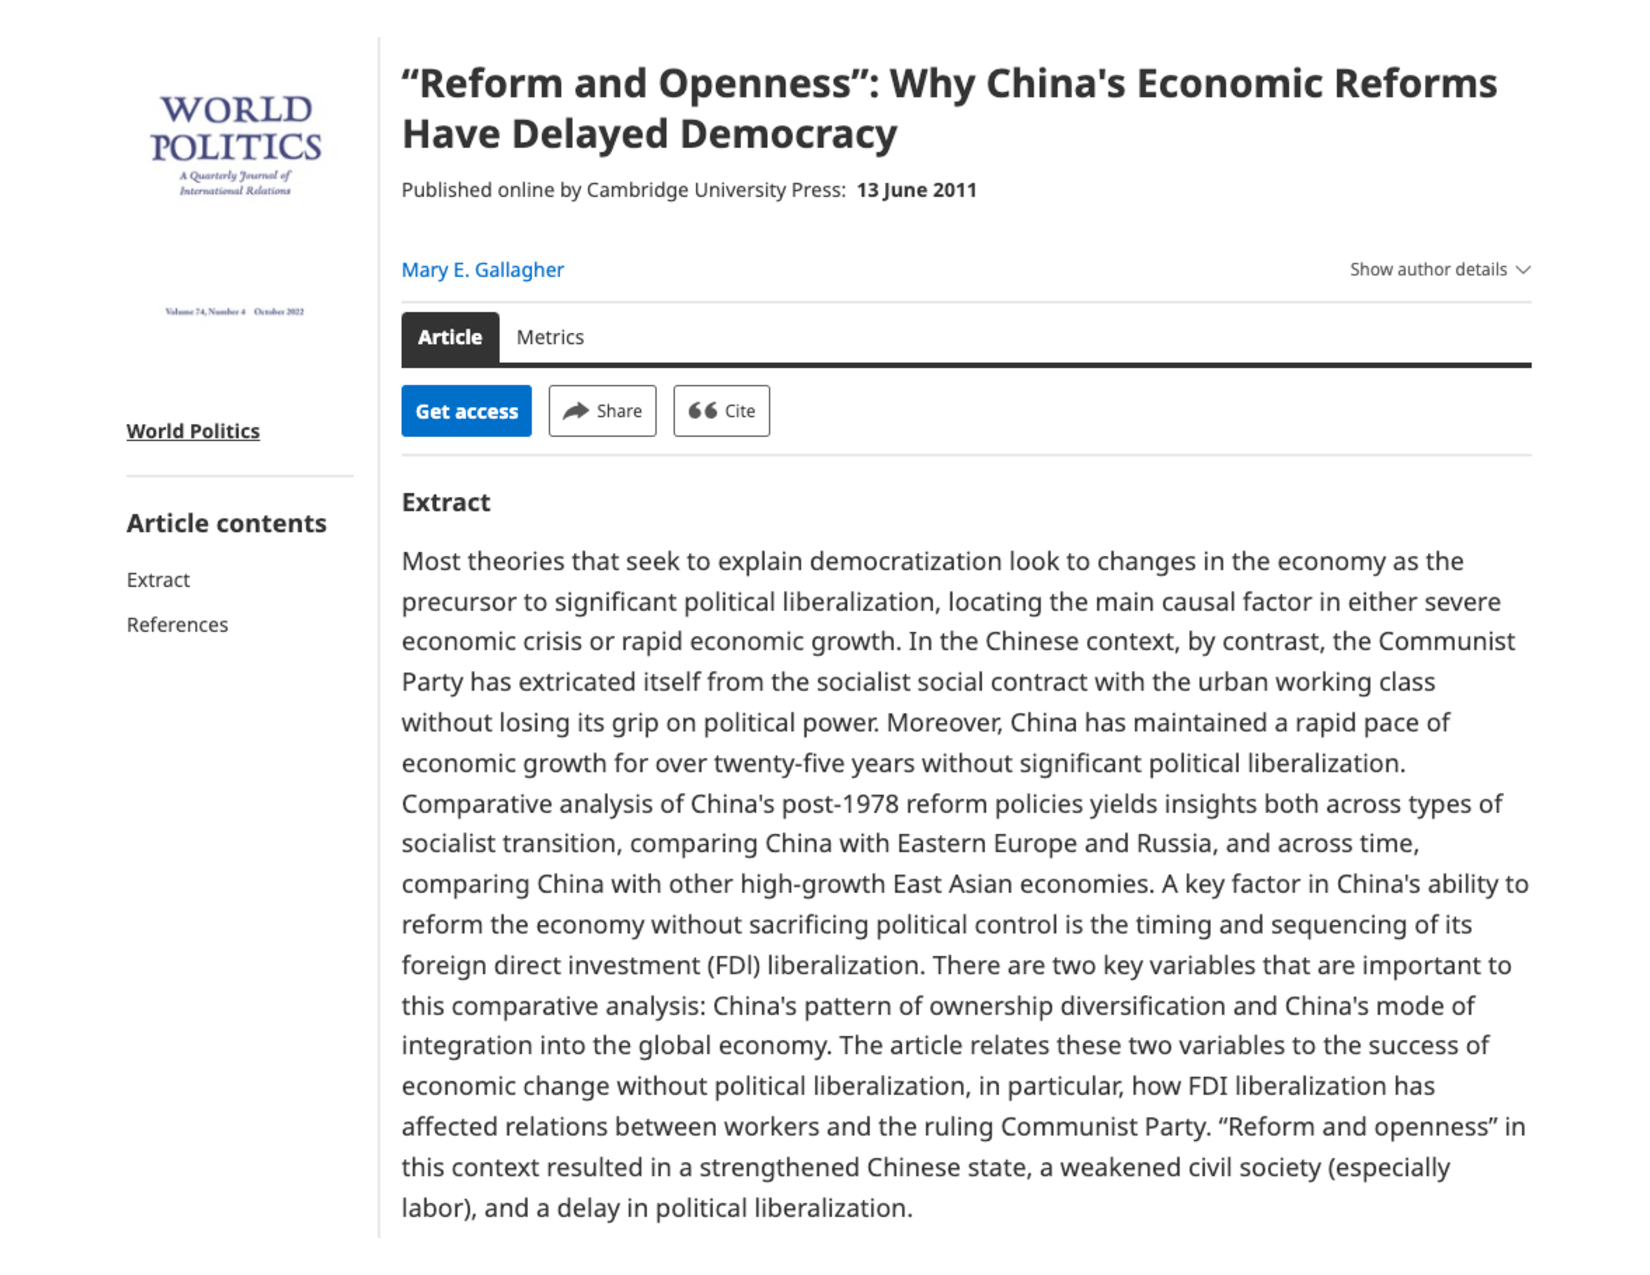
\includegraphics[width=1\linewidth]{Figs/mary} \end{center}
\end{frame}

\begin{frame}
\begin{center}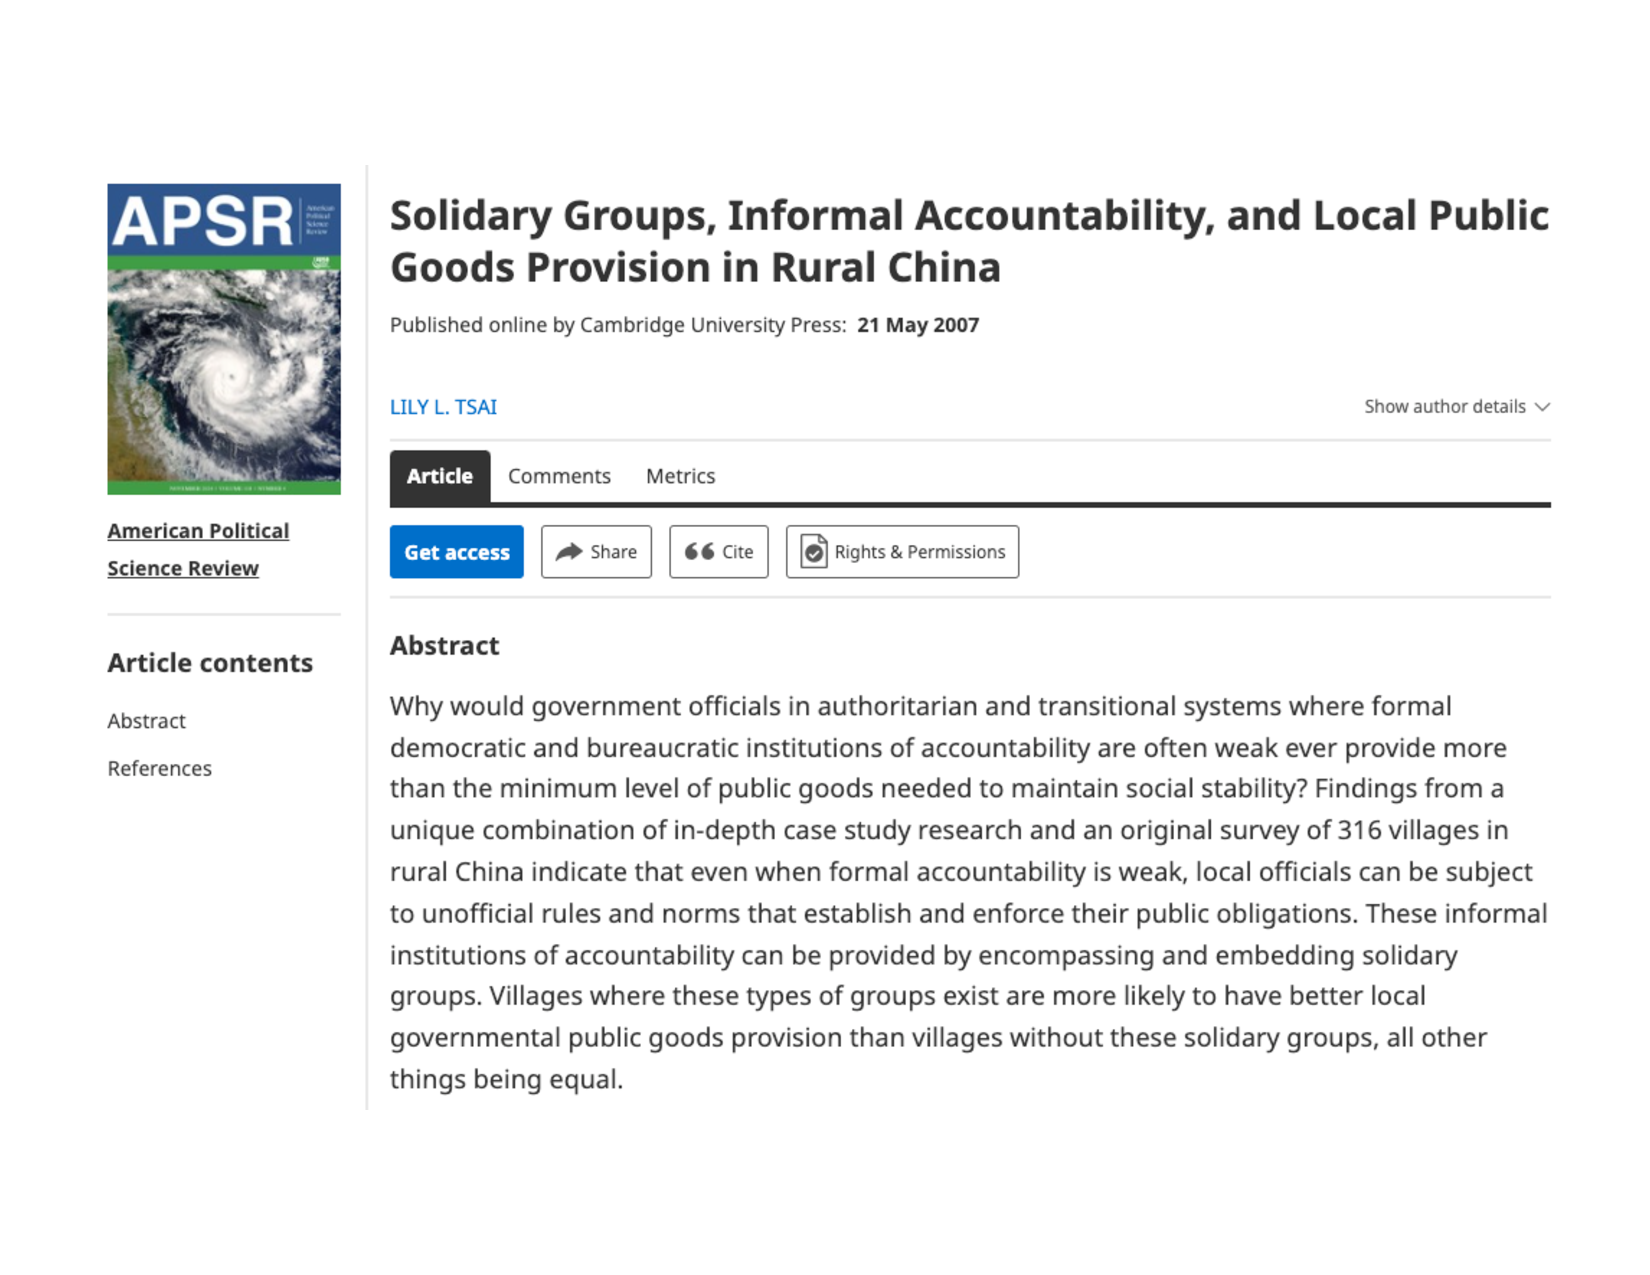
\includegraphics[width=1\linewidth]{Figs/tsai} \end{center}
\end{frame}

\begin{frame}
\begin{center}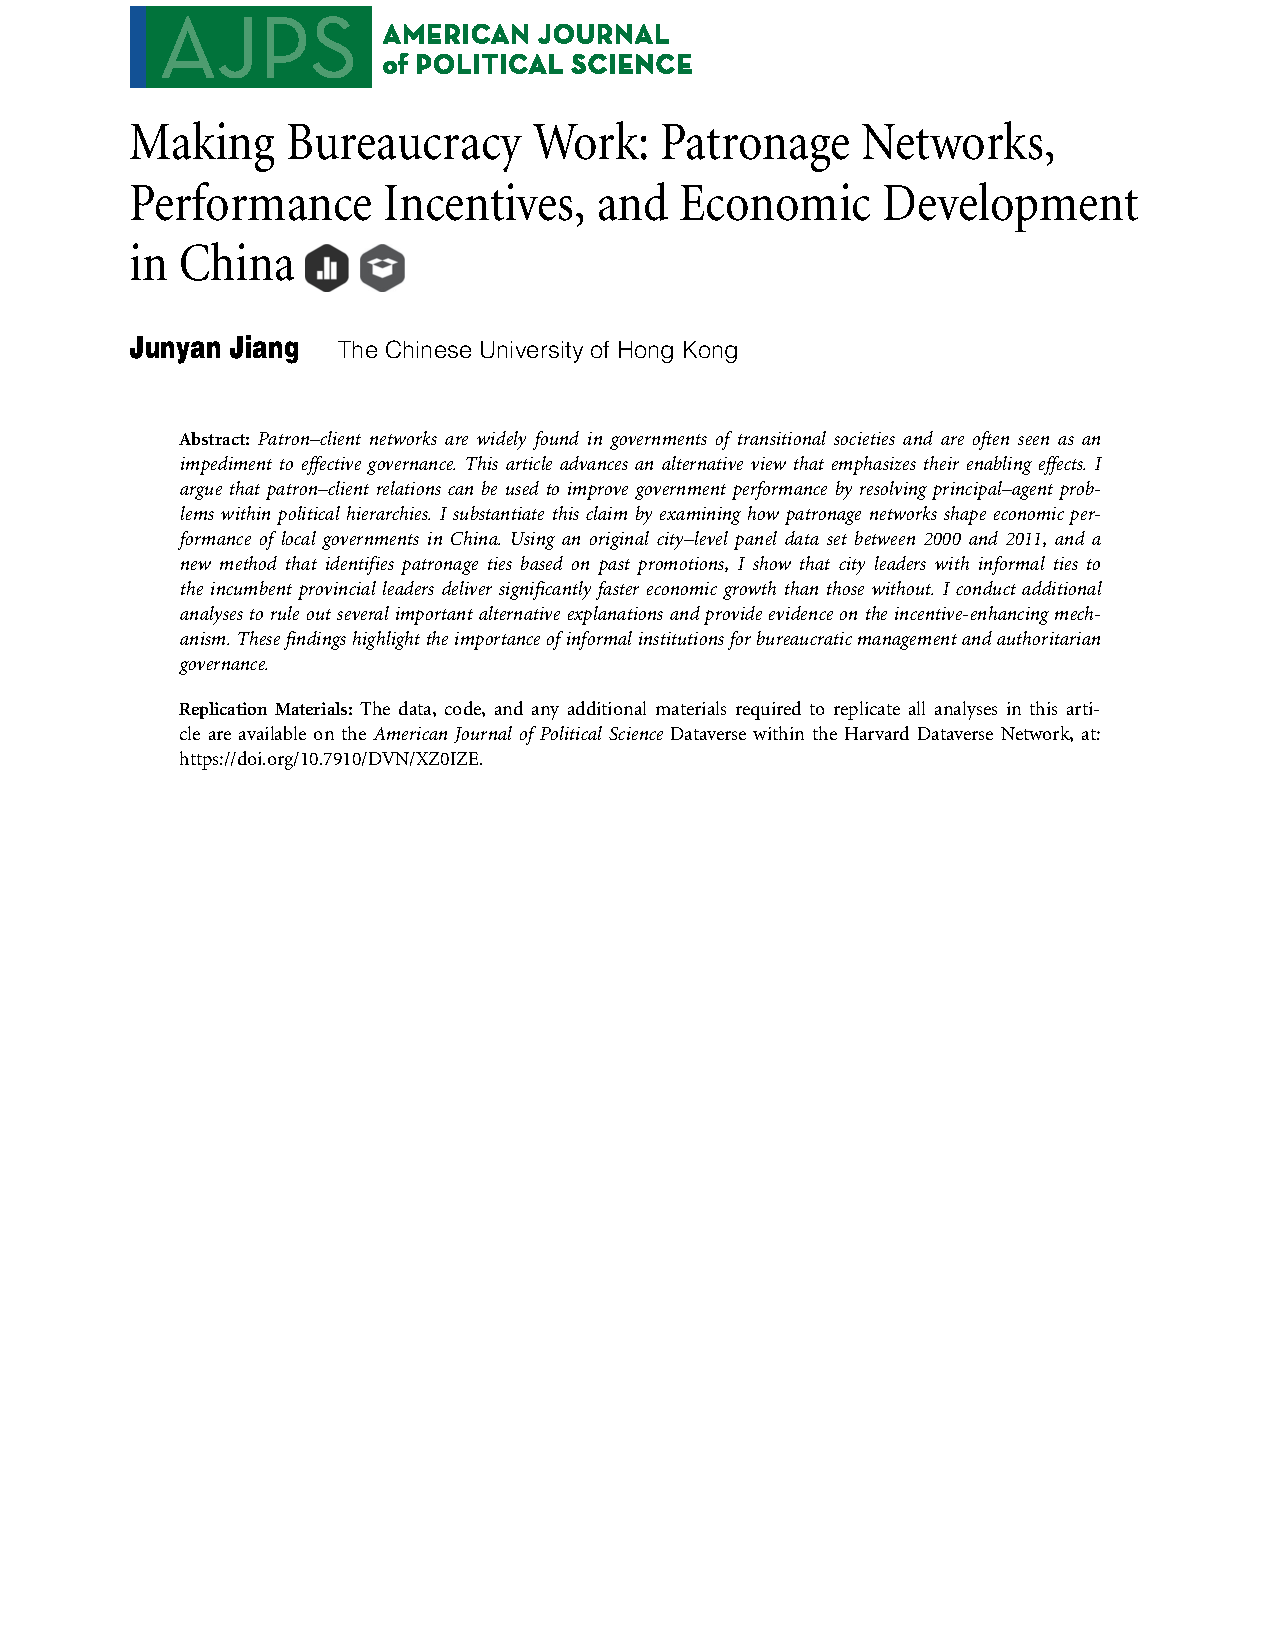
\includegraphics[width=0.95\linewidth]{Figs/jiang} \end{center}
\end{frame}

\begin{frame}
\begin{itemize}
  \item From intelligence services to academic research
  \vspace{0.3cm}
  \item From area studies to comparative politics
  \vspace{0.3cm}
  \item From qualitative description to data-intensive inference
  \vspace{0.1cm}
  \begin{itemize}
    \item Before the diplomatic reconciliation between PRC and USA (1971-1978), scholars have to rely on limited, parrial and often biased qualitative evidence (archives and interviews)
    \item After Reform and Opening, in the 1980s more engaging field research is likely (ethnography and case studies)
    \item The mid-1990s saw the quantitative turn of China studies (surveys, econometric analysis of admin data and computational)
  \end{itemize}
\end{itemize}
\end{frame}

\begin{frame}
\begin{center}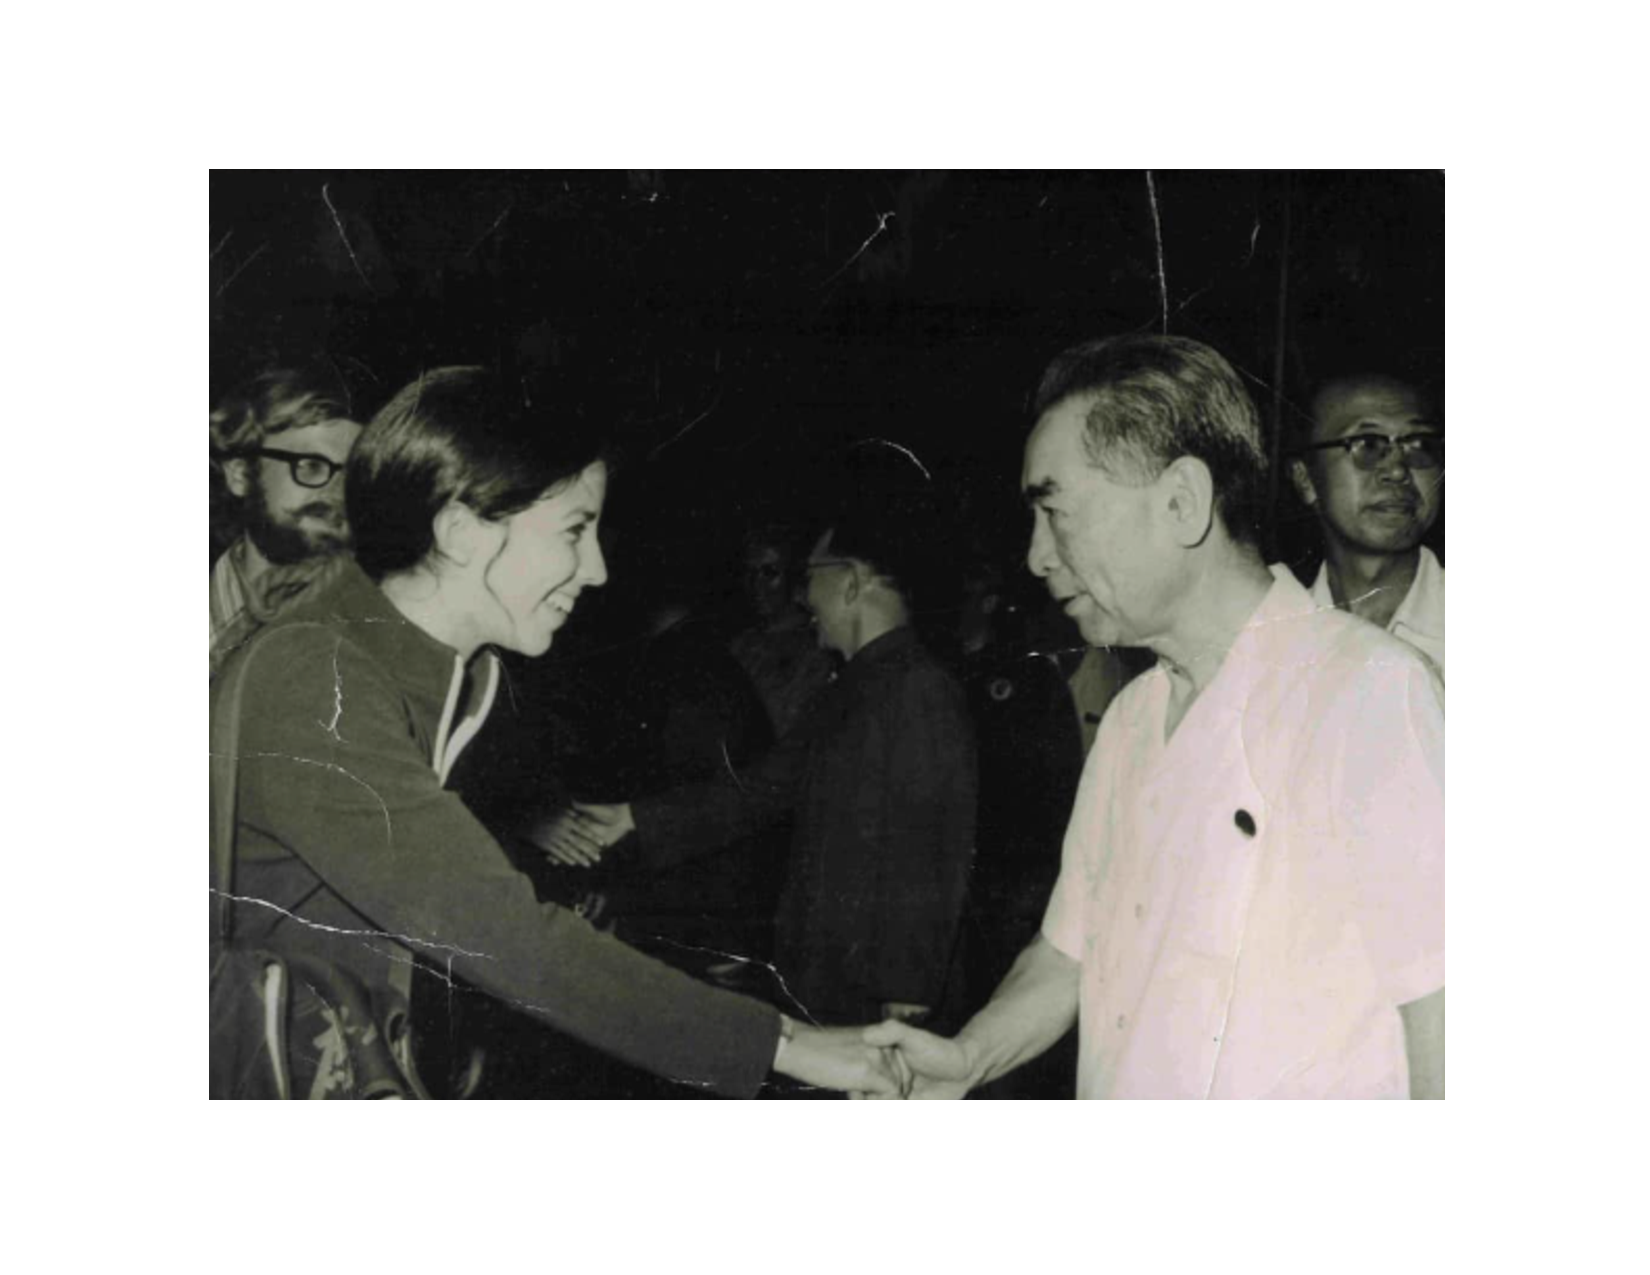
\includegraphics[width=0.9\linewidth]{Figs/shirk71} \end{center}
\vspace{0.1cm}
\begin{center}
\scriptsize
\small
Susan Shirk (UCSD) with Zhou Enlai in July 1971, on a visit to China with "the Committee of Concerned Asian Scholars"
\end{center}
\end{frame}

\begin{frame}
\begin{center}
\textbf{Week 2: Empire to Nation-State}
\end{center}
\vspace{0.3cm}

\begin{center}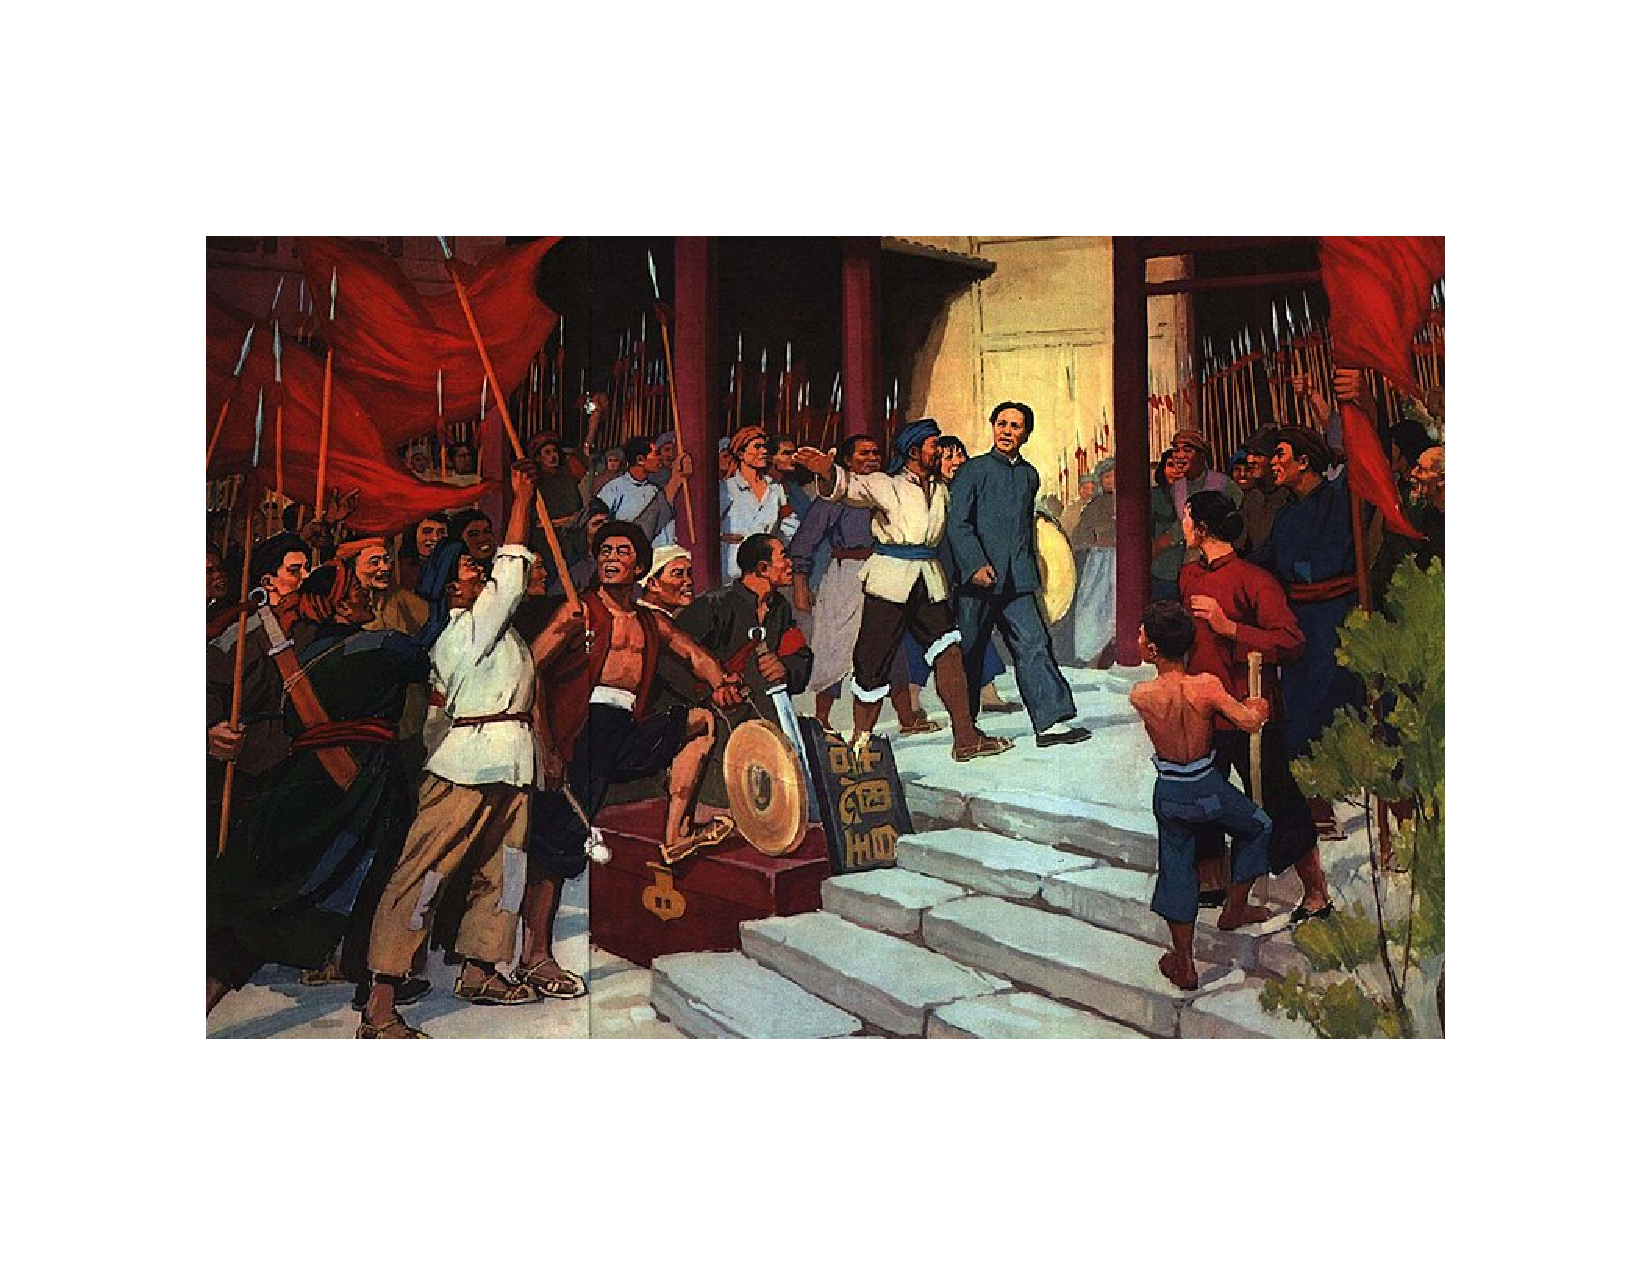
\includegraphics[width=0.7\linewidth]{Figs/theme2} \end{center}
\begin{center}
\footnotesize
\url{https://storystudio.tw/article/gushi/the-forbidden-garden}
\end{center}
\end{frame}

\begin{frame}{``China: A Century of Revolution''}
\protect\hypertarget{china-a-century-of-revolution}{}
\begin{center}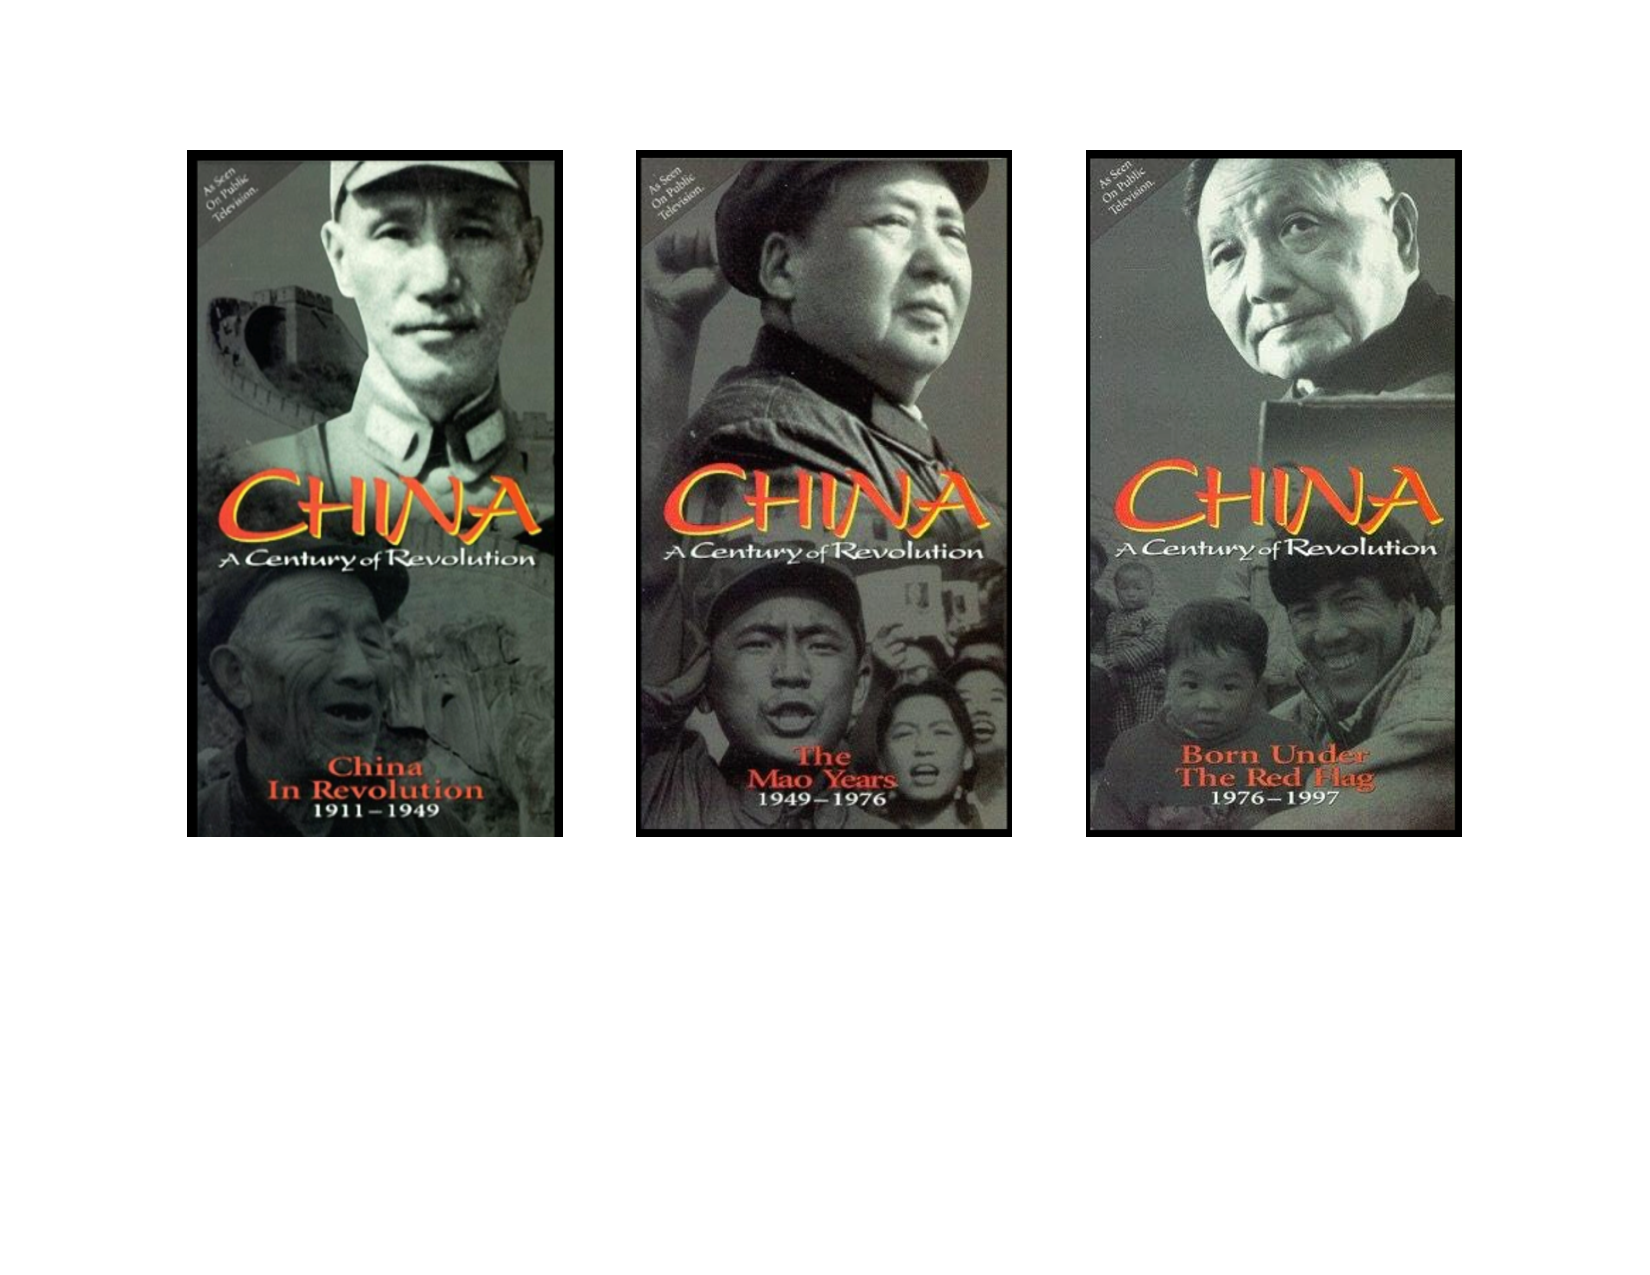
\includegraphics[width=0.95\linewidth]{Figs/docs} \end{center}
\end{frame}

\begin{frame}{China in the 20th century}
\protect\hypertarget{china-in-the-20th-century}{}
\begin{itemize}
  \item Republican China (1911-1949)
  \vspace{0.2cm}
  \begin{itemize}
    \item 1911-1928: Beiyang Government (北洋政府)
    \item 1928-1949: Nationalist/KMT Government (民国政府) 
  \end{itemize}
  \vspace{0.4cm}
  \item Communist China (1949-present)
  \vspace{0.2cm}
  \begin{itemize}
    \item 1950s: Land reform and the Great Leap Forward (大跃进)
    \item 1960s: Return of Mao Zedong and the Cultural Revolution (文化大革命)
    \item 1970s: Power transition and "Reform and Opening" (改革开放)
    \item 1980s: Experiment with market economy, intra-party split and Tiananmen
    \item 1990s: Consolidated market reform and institutionalized political succession (?)
  \end{itemize}
\end{itemize}
\end{frame}

\begin{frame}
\vspace{1cm}

See you next week!
\end{frame}

\end{document}
